% ============================================================================
% Stream: Token-Free Byte-Level State Space Language Models
% arXiv-style submission. Compile with pdflatex (2 passes) or latexmk.
% Requires: amsmath, amssymb, graphicx, booktabs, caption, xcolor,
%           hyperref, geometry — all standard on arXiv / TeX Live / MiKTeX.
% ============================================================================
\documentclass[11pt]{article}

\usepackage[utf8]{inputenc}
\usepackage[T1]{fontenc}
\usepackage{textcomp}
\usepackage{geometry}
\geometry{margin=1in}

\usepackage{amsmath,amssymb}
\usepackage{graphicx}
\usepackage{booktabs}
\usepackage{xcolor}
\usepackage{caption}
\usepackage[bookmarks=false,hidelinks]{hyperref}
\emergencystretch=3em

\newcommand{\loss}{\mathcal{L}}
\newcommand{\Stream}{\texttt{Stream}}
\newcommand{\StreamR}{\texttt{StreamR}}
\newcommand{\StreamD}{\texttt{StreamD}}
\newcommand{\Vector}{{\scshape Vector}}
\newcommand{\voc}{v_{\text{voc}}}

\title{\bfseries Stream: Token-Free Byte-Level State Space Language Models\\
       \large with Honest Measurements of Scaling, Linear-Time Decoding, and Loss Trade-offs}

\author{
  \textbf{Nishant}\\[2pt]
  \normalsize Independent Researcher \\[2pt]
  \normalsize \texttt{RETRANS-X} project \\[4pt]
  \normalsize GitHub: \url{https://github.com/nishantXnova/RETRANS-X}
}

\date{August 2026}

\begin{document}

\maketitle

% ============================================================================
\begin{abstract}
\noindent
We introduce \Stream{}, a token-free, position-free language model built entirely
on selective state space (SSM) recurrence that operates directly on raw UTF-8
bytes with a fixed vocabulary of 256 byte values. \Stream{} removes the entire
tokenization pipeline (no BPE, no WordPiece, no SentencePiece), removes
positional encoding (position is encoded structurally by the sequential scan),
and retains $O(n)$ time and $O(n)$ memory complexity in sequence length. The
architecture is a 256-entry byte embedding followed by Mamba-style selective
SSM blocks and a multi-byte prediction head that predicts four future bytes per
position simultaneously. We additionally release the \texttt{SSMScanFn} primitive,
a JIT-compiled custom-autograd linear-time scan whose manual backward pass avoids
the $O(T^2)$ autograd graph overhead, together with fused and chunked Triton
kernels that bring end-to-end training within $\sim$5$\times$ of a hand-optimized
JIT loop and deliver flat $\sim$228\,K\,bytes/s throughput from $T=512$ to
$T=16{,}384$ on a single Tesla T4.

Empirically, on raw bytes of TinyStories, \Stream{} at 4.43\,M parameters reaches
1.69 byte-level validation cross-entropy, within $\sim$0.5\,nats of a
similarly-sized Transformer at the matched-parameter budget. In a carefully
matched byte-level head-to-head (identical data, schedule, and batch at
$T=4096$), \Stream{} \emph{leads} the Transformer for roughly the first 2{,}500
iterations and finishes within 0.39 nats at 5{,}000 iterations while predicting
four bytes ahead and using 26\% fewer parameters. Memory usage scales exactly
linearly with context (6.77\,GB peak at $T=65{,}536$ on a 15\,GB GPU), and the
O(n)/O(n$^2$) wall-time crossover is empirically validated at $T\approx 9$\,k,
where \Stream{} becomes 1.73$\times$ faster than Transformer attention at
$T=16{,}384$ and is projected $\sim$3.5$\times$ faster at $T=32{,}768$.

We also report three extensions and their honest negative/blocked results:
\Vector{}, which augments \Stream{} with a learned saliency-gate for position
pruning, grouped-query attention, and mixture-of-experts layers under a
five-term loss, whose gate collapses to ``keep everything'' ($\text{active ratio}\equiv1.0$)
-- a diagnosed and fixable optimization-landscape failure, not an architectural
dead end; \Stream{}-MoE, a sparse mixture-of-experts variant with
gradient-aware expert lifecycle management, where automatic expert replacement
currently \emph{hurts} validation loss (2.35 vs.\ 2.19) because gradient-based
impact is too noisy in early layers; and \StreamR{}, a \Stream{} whose last SSM
blocks are replaced by sparse-retrieval attention (sliding-window $+$ static
global tokens, $O(n)$ memory) targeting content-based recall, whose 4-layer
pilot matches \Stream{} at short context and whose long-context verdict is
pending at submission; with a pure-recurrence counterpart, \StreamD{}
(Section~\ref{sec:streamd}), whose content-addressed delta matrices are the
bounded-attention-free hypothesis for the same verdict. All code, configs,
and scripts for reproducing every
table and figure are released; the full reproducibility playbook is included in
Section~\ref{sec:repro}.
\end{abstract}

% ============================================================================
\section{Introduction}\label{sec:intro}

The Transformer \cite{Vaswani2017Attention} has dominated natural language
processing for nearly a decade, but its reliance on discrete subword
tokenization carries a set of cascading design burdens: a fixed vocabulary of
tens of thousands of entries, lossy byte-to-token mappings, tokenizers trained
on English-heavy corpora that under-serve low-resource languages, and an
explicit positional-encoding ``band-aid'' for the permutation-invariance of
attention. These choices have concrete costs -- $O(n^2)$ attention in token
count, information loss from byte-to-token compression, brittle cross-lingual
transfer, and a separate engineering pipeline for every new language
\cite{Xue2021ByT5,Clark2022CANINE}.

State space models (SSMs) offer a different decomposition. The Structured State
Space sequence model (S4) \cite{Gu2021S4} and its selective successors Mamba
\cite{GuDao2023Mamba} and Mamba-2 \cite{DaoGu2024Mamba2} retain a linear
recurrence $h_t=\bar A_t h_{t-1}+\bar B_t x_t$ while allowing input-dependent
transition matrices, matching or approaching Transformer quality on language
modeling at $O(n)$ inference cost. Crucially, the recurrence is inherently
sequential: position is encoded by the scan itself, so no positional encoding is
needed. MambaByte \cite{Wang2024MambaByte} demonstrated that this paradigm can
be pushed to its logical extreme -- operating directly on raw bytes without any
tokenizer.

\paragraph{This work.}
We develop and honestly characterize \Stream{}, a token-free byte-level SSM
language model. \Stream{} is simultaneously:
\begin{itemize}
  \item \textbf{Token-free}: vocabulary $=$ 256 byte values, no BPE/WordPiece/SentencePiece;
  \item \textbf{Position-free}: the SSM recurrence is the positional signal;
  \item \textbf{Segmentation-free}: the model observes every byte and learns
        boundaries end-to-end;
  \item \textbf{$O(n)$ compute and memory} in sequence length.
\end{itemize}

Beyond presenting the architecture, the contributions of this work are
technical and empirical:

\begin{enumerate}
  \item \textbf{\texttt{SSMScanFn}, a custom-autograd linear-time scan.} The
        forward pass runs $h_{t+1}=a_t h_t+b_t$ in $O(T)$; the manual backward
        pass runs a reverse scan producing $\partial\loss/\partial a$ and
        $\partial\loss/\partial b$ in $O(T)$ without materializing the $O(T)$
        autograd graph, and JIT compilation fuses the per-step elementwise ops
        into single kernels, eliminating per-step Python and kernel-launch
        overhead.
  \item \textbf{Fused and chunked Triton scans.} On hardware, the naive loop is
        the bottleneck, not the recurrence. We contribute a fused Triton kernel
        (computing $\exp(\Delta_t A)$ and $\Delta_t B u$ in registers so the
        $(B,T,H,N)$ intermediates are never materialized) and a chunked
        two-level scan for the occupancy-starved low-$B\cdot H$ regime, with a
        shape-conditional dispatch rule ($B\cdot H\le128$ picks chunked) backed
        by measured T4 data. Together these deliver a $\sim$5$\times$
        end-to-end training speedup over the JIT loop and flat $O(n)$
        throughput (Section~\ref{sec:gpu}).
  \item \textbf{Multi-byte prediction.} Each position predicts the next
        $\mathrm{n\_predict}=4$ bytes, giving 4$\times$ training-signal density
        and 4$\times$ faster autoregressive decoding -- a critical compensation
        for the higher per-step entropy of byte-level prediction.
  \item \textbf{A measured, honest account of the token-free accuracy gap.}
        We quantify the byte-level cost: $\approx$0.5 nats at matched small
        budgets, with the gap closing or reversing in matched byte-level
        head-to-heads and at long context (Section~\ref{sec:mainresults}).
  \item \textbf{Documented external/extended designs.} \Vector{} (learned
        position pruning + attention + MoE under a five-term loss) and
        \Stream{}-MoE (gradient-aware expert lifecycles), including the
        diagnosis of \Vector{}'s gate collapse and \Stream{}-MoE's negative
        replacement result (Section~\ref{sec:extensions}).
\end{enumerate}

The central question we investigate is: \emph{how much modeling capacity is
lost by operating on raw bytes instead of learned subword tokens, and can the
efficiency gains of linear-time recurrence compensate?} Our answer is measured
rather than asserted: \Stream{} converges and produces coherent, tokenizer-free
byte-level language models; the Transformer retains a loss advantage at small
matched budgets; but \Stream{}'s $O(n)$ wall-time and $O(n)$ memory are real on
consumer hardware and its loss gap narrows -- and on matched byte-level data,
its lead at intermediate training budgets is real.

% ============================================================================
\section{Related Work}\label{sec:related}

\paragraph{State space sequence models.}
S4 \cite{Gu2021S4} introduced efficient diagonal SSMs; Mamba \cite{GuDao2023Mamba}
added input-dependent (selective) transitions, closing the gap to Transformers
on language modeling; Mamba-2 \cite{DaoGu2024Mamba2} unified SSMs and attention
through state-space duality and added tensor-parallel training. Our recurrence
follows the Mamba block structure (input projection, depthwise conv, selective
scan, output projection with residual + layernorm), and \texttt{SSMScanFn} is a
pure-PyTorch implementation of the same insight that makes Mamba's CUDA kernel
efficient -- a manual backward recurrence instead of an autograd graph.

\paragraph{Token-free language modeling.}
ByT5 \cite{Xue2021ByT5} and CANINE \cite{Clark2022CANINE} process bytes/chars
with Transformers but inherit $O(n^2)$ attention at byte granularity; MegaByte
\cite{Yu2023MegaByte} uses hierarchical multiscale Transformers for
million-byte sequences. Most directly, MambaByte \cite{Wang2024MambaByte}
showed a selective SSM can match a byte-level Transformer (MegaByte) in quality
while being more efficient. \Stream{} builds on this result and contributes
multi-byte prediction, fused linear-time scans with measured GPU behavior, and
a careful quantification of the byte-level gap against a standard Transformer
baseline on identical data.

\paragraph{Sparse and dynamic computation.}
The sparse mixture-of-experts (MoE) paradigm \cite{Shazeer2017MoE},
Switch Transformers \cite{Fedus2021Switch}, and ST-MoE \cite{Zoph2022STMoE}
scale capacity without proportional FLOPs. Studies of dead-expert detection and
replacement \cite{Roller2021Evolving,Kim2023Expert} typically use router
frequency or confidence heuristics. Our \Stream{}-MoE instead scores experts by
a gradient-derived impact-to-frequency ratio and reports a controlled negative
result for the replacement mechanism at small scale. Learned conditional
computation and gradient estimators \cite{Bengio2013STE} underpin \Vector{}'s
straight-through-estimated saliency gate. We also use grouped-query attention
\cite{Ainslie2023GQA} inside \Vector{}.

% ============================================================================
\section{The \Stream{} Architecture}\label{sec:stream}

\Stream{} is the simplest byte-level SSM language model we could design. The
full dataflow is shown in Figure~\ref{fig:arch},
\begin{equation}
\text{bytes } b_{1:T}\in[0,255]
\xrightarrow{\text{Embed}_{256\to d}}
[\text{SSMBlock}]^{\times L}
\xrightarrow{\text{Multibyte head}}
\hat b_{t+1},\dots,\hat b_{t+\mathrm{n\_predict}}.
\end{equation}

\begin{figure}[t]
  \centering
  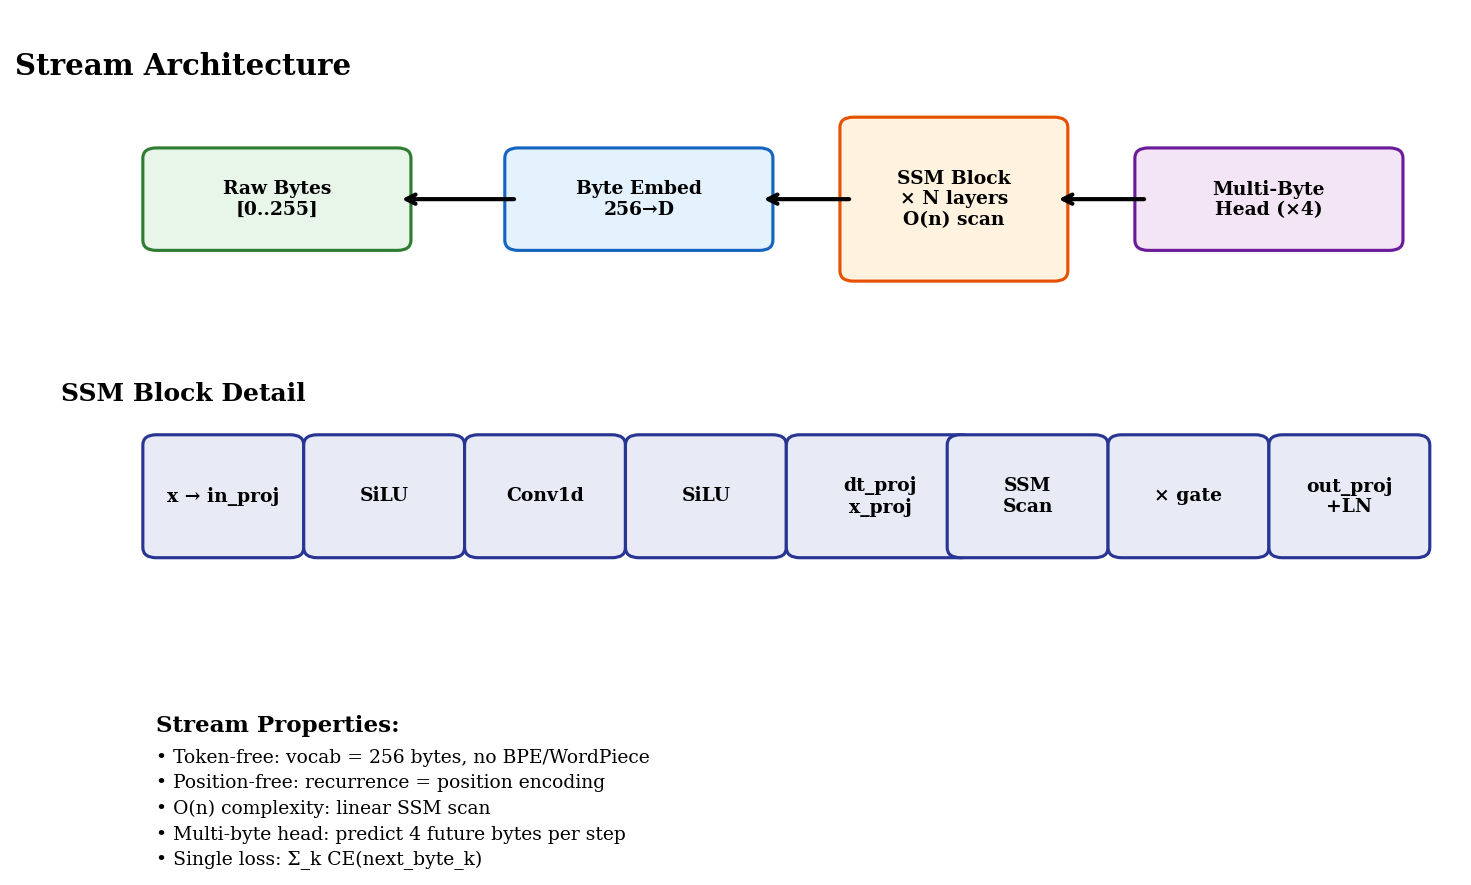
\includegraphics[width=0.92\textwidth]{figures/fig1_architecture.png}
  \caption{The \Stream{} architecture and SSM block detail.}
  \label{fig:arch}
\end{figure}

\subsection{Byte embedding}
The input is a raw byte sequence $b_1,\dots,b_T$, $b_t\in\{0,\dots,255\}$, mapped
through a learned $256\times d$ lookup table $x_t=\text{Embed}(b_t)$. This
256-entry table is the entire ``vocabulary'' of the model; there are no merge
tables, no unigram models, and no language-specific preprocessing.

\subsection{Selective SSM block}
Each block follows Mamba's design \cite{GuDao2023Mamba}. Given hidden dimension
$d$ and state size $n$:
\begin{itemize}
  \item input projection $d\to 2d_{\text{hidden}}$ split into a main branch and a
        SiLU-gated branch;
  \item a depthwise 1-D convolution (kernel 4, groups $=d_{\text{hidden}}$) with
        SiLU;
  \item the selective scan with learned, input-dependent step size
        $\Delta_t=\text{softplus}(W_\Delta x_t)$,
        \begin{equation}
          a_t=\exp(\Delta_t A),\quad b_t=\Delta_t B_t x_t,\qquad
          h_t=h_{t-1}\,a_t+b_t,\quad y_t=\text{sum}_n(h_t\odot C_t)+D\,x_t,
          \label{eq:scan}
        \end{equation}
        where $A=-\exp(A_{\text{log}})$ is a diagonal (log-space) state matrix so
        the recurrence is always stable;
  \item output projection back to $d$, SiLU gating, residual connection, and
        final layer normalization.
\end{itemize}

Because Equation~\eqref{eq:scan} is sequential, position is structural: no
positional encoding is ever added, and dropping it does not make the model
position-blind.

\subsection{\texttt{SSMScanFn}: custom-autograd linear scan}
\label{sec:triton}
The recurrence in Equation~\eqref{eq:scan} is implemented once as a
JIT-compiled forward/backward pair wrapped by a custom
\texttt{torch.autograd.Function}:
\begin{itemize}
  \item the \emph{forward} loop runs $h_t=h_{t-1}a_t+b_t$ for $t=1..T$, storing
        the trajectory;
  \item the \emph{backward} loop runs the reverse recurrence
        $\mathrm{dh}_t=\partial\loss/\partial h_t+\mathrm{dh}_{t+1}$, emitting
        $\partial\loss/\partial a_t$ and $\partial\loss/\partial b_t$ directly
        in $O(T)$ time and $O(T)$ memory.
\end{itemize}
The custom backward avoids building the $O(T)$-node autograd graph that a
naive loop would construct, eliminating $O(T^2)$-equivalent bookkeeping on long
sequences. On CPU the sequential loop is also optimal; JIT compilation fuses
per-step elementwise ops into a single kernel so there is no per-step Python
dispatch. On GPU the same \texttt{SSMScanFn} graph is used, but the per-step
kernels are replaced by the fused/chunked Triton scans described in
Section~\ref{sec:triton}.

\subsection{Multi-byte prediction head}
From each position $t$ the head maps $d\to\mathrm{n\_predict}\times256$ logits
and predicts $b_{t+1},\dots,b_{t+\mathrm{n\_predict}}$ with
\begin{equation}
\loss=\frac{1}{\mathrm{n\_predict}}\sum_{k=1}^{\mathrm{n\_predict}}
\text{CE}(\text{logits}_{t,k},\,b_{t+k}).
\label{eq:loss}
\end{equation}
This gives 4$\times$ training-signal density per position and 4$\times$ faster
autoregressive decoding (one forward pass emits four bytes). We found this to be
important in practice: byte-level next-byte entropy is higher than token-level
next-token entropy, and the $k$-step objectives add a cheap n-gram-like bias.
Figure~\ref{fig:multibyte} illustrates the head.

\begin{figure}[t]
  \centering
  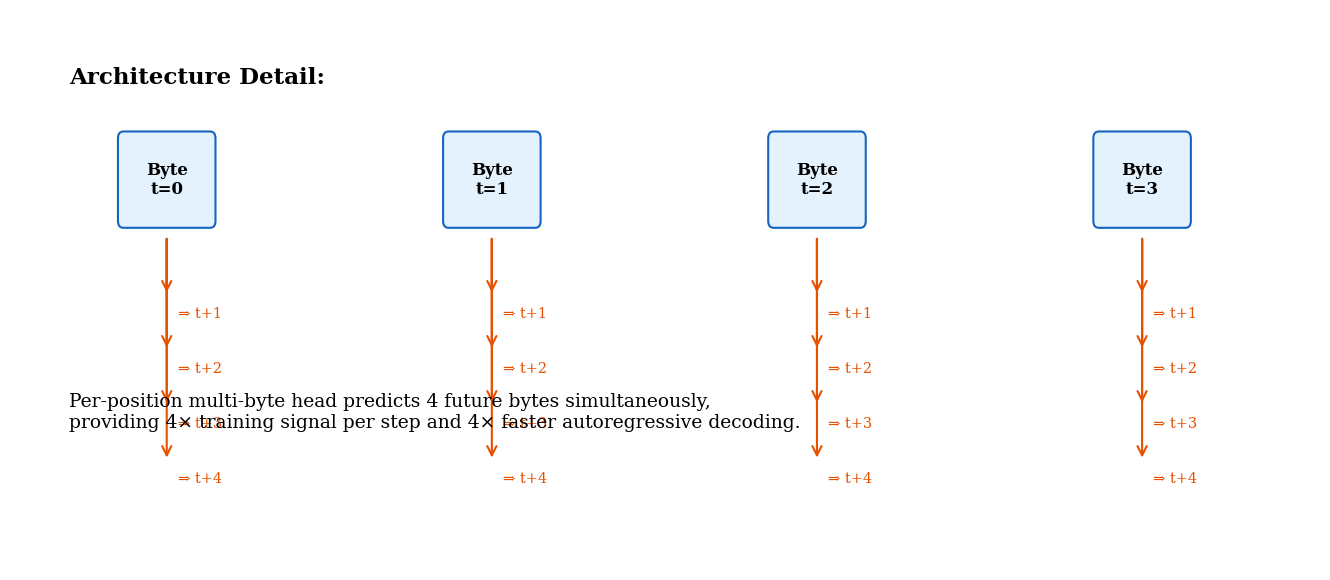
\includegraphics[width=0.92\textwidth]{figures/fig7_multibyte.png}
  \caption{The multi-byte prediction head: four future bytes predicted per
  position.}
  \label{fig:multibyte}
\end{figure}

\subsection{Training objective}
\Stream{} uses exactly one loss term, Equation~\eqref{eq:loss}: cross-entropy
over predicted bytes summed across the prediction horizon. This single-objective
design keeps training stable and results interpretable, and distinguishes
\Stream{} from the multi-loss \Vector{} architecture below.

% ============================================================================
\section{Extensions and Their Honest Results}\label{sec:extensions}

To contextualize \Stream{}, we evaluate three extensions that were developed in
the same codebase: \Vector{}, a position-pruning architecture with attention and
MoE; \Stream{}-MoE, a sparse-MoE variant with expert lifecycle management; and
\StreamR{}, a \Stream{} that replaces its last SSM blocks with sparse-retrieval
attention to close the content-based-recall gap against Transformers.

\subsection{\Vector{}: saliency-gated position pruning}\label{sec:vector}
\Vector{} adds three components over the SSM backbone: (1) a \emph{saliency
gate} that learns a per-dimension importance threshold $\theta$ and, via a
straight-through estimator \cite{Bengio2013STE}, produces a hard 0/1 mask to
prune low-salience positions toward a target effective length $C_{\text{target}}$;
(2) \emph{AtomAttention}, a grouped-query attention \cite{Ainslie2023GQA} layer
attending only to retained ``atoms''; and (3) an MoE FFN with the Switch-style
load-balance auxiliary loss \cite{Fedus2021Switch}. It is trained with a
five-term loss
\begin{equation}
\loss=\underbrace{\loss_{\text{pred}}}_{=1}
+\alpha\loss_{\text{recon}}+\beta\loss_{\text{budget}}
+\gamma\loss_{\text{anchor}}+\loss_{\text{balance}},
\end{equation}
with reconstruction on pruned positions, a budget-loss on active ratio, and a
between-layer cosine anchor loss.

\paragraph{Gate collapse (documented failure).}
Controlled runs (2L/64D, 0.45M params, 1000 iters, TinyStories bytes) show the
saliency gate learns \emph{not} to prune: active ratio stays at $1.0$ throughout
training, with or without the gate engaged (bypass vs.\ real gate both reach
$\approx$3.57 byte-level val loss -- see Table~\ref{tab:bakeoff}). We diagnose
three interacting causes:
\begin{enumerate}
  \item \emph{Zero pruning pressure during warmup}: budget weight $\beta$ ramps
        from 0, so gate threshold parameters never move from initialization;
  \item \emph{The hinge budget loss vanishes once under budget}:
        $\loss_{\text{budget}}=\text{ReLU}(T_{\text{eff}}-C_{\text{target}})$
        supplies zero gradient once $T_{\text{eff}}\le C_{\text{target}}$, while
        $\loss_{\text{pred}}$ always profits from additional information;
  \item \emph{No countervailing force} pushes atoms out when
        $T_{\text{eff}}<C_{\text{target}}$.
\end{enumerate}
This is a loss-landscape equilibrium at ``keep everything'', not an
architectural dead end. We identify a concrete remediation -- a two-sided
budget penalty $(T_{\text{eff}}-C_{\text{target}})^2$ and/or an entropy bonus on
the router -- as future work (Section~\ref{sec:future}). We also note honestly
that an earlier \Vector{} 3L/128D number (2.98) was produced while the ``gate
bypass'' flag did not actually bypass the gate; those runs measured a randomly
gated model, not a clean \Vector{} baseline, and are not treated as converged
results here.

\subsection{\Stream{}-MoE: gradient-aware expert lifecycles}\label{sec:moe}
\Stream{}-MoE inserts a top-$k$ MoE FFN ($k=2$) after each SSM block and adds
gradient-aware expert lifecycle management. Each expert $i$ maintains two EMAs,
frequency $\text{freq}_i$ and gradient-derived impact
$\text{impact}_i=\text{EMA}(-\partial \loss/\partial y\cdot y)$, captured by
backward hooks on the expert output layer, and a value score
$\text{value}_i=\text{impact}_i/(\text{freq}_i+\varepsilon)$ with empirical-Bayes
shrinkage toward the population mean. Experts whose value score falls below an
adaptive threshold past a probation period are candidates for replacement by
cloning the best expert in the layer with Gaussian noise
($\sigma=0.01$), an exploration bias, and cleared AdamW momentum state. Safety
measures keep the best expert non-replaceable, cap replacements at half the
experts per check, and protect recently-replaced experts with a birth-age bonus.

\paragraph{Replacement ablation (negative result).}
\begin{table}[t]
  \centering
  \small
  \begin{tabular}{lccccc}
    \toprule
    Config & Trigger & Params & Val Loss & Experts replaced \\
    \midrule
    Replacement OFF & --- & $\sim$2.95M & \textbf{2.19} & 0 \\
    Replacement ON & $\theta{=}0.05$, 400 iters & $\sim$2.95M & 2.35 & $\sim$2--4/check \\
    Replacement TUNED & $\theta{=}0.01$, 1000 iters & $\sim$2.95M & 2.19 & 0 (effectively OFF) \\
    \bottomrule
  \end{tabular}
  \caption{\Stream{}-MoE 4L/128D, 4 experts, top-2, 2000 iters on TinyStories
  bytes, $T{=}256$. Automatic expert replacement hurts validation loss.}
  \label{tab:moeab}
\end{table}
As shown in Table~\ref{tab:moeab}, automatic expert replacement \emph{hurts}
validation loss (2.35 vs.\ 2.19 at 2,000 iters on TinyStories bytes). The cause
is specific: gradient-based impact measurements in early SSM layers are noisy --
all four experts in layer~0 registered loss-increasing impacts mid-training,
triggering aggressive false-kills. Tuning the threshold stricter simply
disabled replacement, matching the ``OFF'' baseline. We therefore keep
replacement disabled by default in all shipped configs and treat this as a
controlled negative result: meaningful lifecycle management likely needs either
pooled impact measurements over larger windows, deferred lifecycle decisions,
or router-entropy-based dead-expert detection.

\subsection{\StreamR{}: sparse-retrieval blocks for content-based recall}\label{sec:streamr}
The matched-budget gap against Transformers (Section~\ref{sec:mainresults})
suggests a fixed $d_{\text{state}}{=}16$ recurrence compresses history but
cannot perform content-based recall -- attention can go back and ``find'' a byte
from $1{,}000$ steps earlier, an SSM cannot. \StreamR{} adds retrieval
\emph{selectively}: most layers remain SSM ($O(n)$), and the last
$n_{\text{retrieval}}$ SSM blocks are replaced by a \texttt{RetrievalBlock}
(\texttt{VECTOR/model.py}). Plain \Stream{} is the special case
$n_{\text{retrieval}}{=}0$, so the swap is config-driven and the model stays
token-free, position-free, byte-level, and $O(n)$ in memory.

\paragraph{RetrievalBlock.}
From hidden state $x\in\mathbb{R}^d$, a $d\to3d$ projection produces $q,k,v$
split into $n_h{=}4$ heads of dimension $d/n_h{=}64$. Windowed keys/values are
formed by left-padding $k,v$ by $w{-}1$ and applying a causal sliding-window
\texttt{unfold} of size $w{=}128$; position $t$ therefore attends to exactly
$[t{-}w{+}1,t]$ by construction, with no triangular mask and no $O(T^2)$ matrix.
Attentions are
\begin{equation}
\ell^{w}_t=\frac{q_t\!\cdot\! k^{\text{win}}_t}{\sqrt{d/n_h}}+\mathrm{rel\_bias}[t{-}t'],
\qquad
\ell^{g}_t=\frac{q_t\!\cdot\! g_k}{\sqrt{d/n_h}},
\end{equation}
where $\mathrm{rel\_bias}\in\mathbb{R}^{2w{-}1}$ is a learned
translation-invariant relative-position bias (keeping the model position-free)
and $g_k,g_v\in\mathbb{R}^{16\times4\times64}$ are \emph{static} learned global
key/value tokens (sink-style memory). The head softmaxes over the $16{+}w{=}144$
slots, and the block finishes with a residual and post-normalization identical
to the SSM block. Memory is $O(B\!\cdot\! d\!\cdot\!T\!\cdot\! w)$, not $O(T^2)$.

\paragraph{Honest pilot (4-layer, short context).}
The only completed run at the time of writing is a 4-layer pilot at
$T{=}4096$ (leg A protocol, JIT + fp32, 1{,}200 steps): \Stream{}-4L reaches
final val loss \textbf{2.0875} at 968.5\,ms/step, while \StreamR{}-4L reaches
\textbf{2.0968} at 1{,}004.6\,ms/step (0.90M vs.\ 0.77M params). Retrieval is
\emph{slightly worse} at short context -- expected, since $w{=}128$ recall only
pays off when the context exceeds the window. The 10M tier (StreamR-10M at
10.44M vs.\ Stream-10M at 11.26M vs.\ GPT-8L at 6.62M; legs A $T{=}4096$ and B
$T{=}16384$, where GPT's $O(n^2)$ attention cannot fit the T4) was queued, not
run, at submission. We report the architecture and protocol now and leave the
long-context verdict as future work (Section~\ref{sec:future}). We also note
two caveats: the global tokens are static (content-derived keys/values are the
natural v2 upgrade), and $w{=}128$ is small, so the 144-slot head is the main
per-block overhead at $T{=}4096$.

\paragraph{RetrievalBlock v2 (content-based, the new default).}
The v2 upgrade replaces the static-global/short-window caveats with three
content-based pathways fused per head, while staying token-free,
position-free, and $O(n)$ in memory:
\begin{itemize}
  \item \emph{Per-head relative bias.} $\mathrm{rel\_bias}$ becomes
        $\mathrm{rel\_bias}_h\in\mathbb{R}^{4\times(2w{-}1)}$, allowing each
        head to specialize its distance preference.
  \item \emph{Strided far window.} Position $t$ also attends to an
        $O(w)$-cost arithmetic-progression template
        $\{t{-}(w{+}1){-}k\,s\}_{k=0}^{K_s{-}1}$ with its own learned bias; a
        head can thus ``skip-scan'' far behind the dense window, with no tokens
        and no $O(n^2)$ matrix.
  \item \emph{Content-derived segment memory.} The sequence is split into
        non-overlapping segments of length $m{=}64$; each segment is pooled by
        attention over a learned per-head query into a key/value (an $O(n)$
        pooling, not $O(n^2)$), and position $t$ attends to the last $K_m$
        segments \emph{strictly before} its own with a learned distance bias.
        This is exactly the ``content-derived keys/values'' upgrade named
        above, so recall no longer depends on the static tokens.
\end{itemize}
The four pathways (window, stride, memory, global) are fused by a learned
per-head softmax gate $\pi_h$ over their scores. Every v2 parameter is few
per head (biases, the pool query, the gate); the segment pool is $O(n)$ by
construction. When all v2 flags are off
($\mathrm{per\_head\_bias}{=}F$, $\mathrm{stride}{=}0$,
$\mathrm{mem\_slots}{=}0$, $\mathrm{gate}{=}F$) the block reduces to v1
\emph{exactly} (asserted by \texttt{check\_retrieval\_v2()}: 0.0 diff,
strict causality, gradient to every new parameter), so the v1 pilot numbers
above remain valid. The default long-context configuration is now
\texttt{VECTOR/config/streamr\_long.py} (StreamR-10M, v1+):
\texttt{n\_embd=256, n\_layer=16, n\_retrieval=2, window\_size=128,
n\_global=16, n\_attn\_head=4, per\_head\_bias=True, retr\_stride=8,
retr\_stride\_slots=32, retr\_mem\_slots=16, retr\_mem\_seg=64,
retr\_gated=True}; it equips the queued long-context A/B verdict
(Section~\ref{sec:repro}).

\subsection{\StreamD{}: gated delta memory (content-addressed recurrence)}
\label{sec:streamd}
\StreamR{} retrieves with \emph{bounded attention}; a competing hypothesis is
that content-addressed recall can be done \emph{recurrently} with no attention
at all. \StreamD{} replaces the last $n_{\text{delta}}$ SSM blocks with a
\texttt{DeltaMemoryBlock} (\texttt{VECTOR/model.py}), whose state is exactly
$n_h$ associative matrices $W_h\!\in\!\mathbb{R}^{h_d\times h_d}$ ---
fixed-size in $T$, updated with the delta rule:
\begin{equation}
\text{read:}\;\; o_t=W_{t-1} q_t, \qquad
\text{write:}\;\; W_t=\lambda_t W_{t-1}+\beta_t\,(v_t-W_{t-1}k_t)\,k_t^{\top},
\label{eq:delta}
\end{equation}
where $\lambda_t,\beta_t\!\in\!(0,1)$ are learned, input-dependent, per-head
decay and write-gain gates (init $\lambda\!\approx\!0.9$ persistent /
$\beta\!\approx\!0.5$), and $k_t$ is RMSNorm-normalized per head so unit-length
keys bound interference and keep the matrix stable in fp16. Reads use the
state \emph{before} the current write, so recall is strictly causal, and the
whole block is token-free, position-free, with no attention and no $O(n^2)$
matrix --- pure recurrence. Like \StreamR{}, this is config-driven:
$n_{\text{delta}}{=}0$ is plain \Stream{}, and the two block families share
the same socket, so the swap is the only difference in the A/B. Optional
hybrid: $d_{\text{window}}{>}0$ adds an exact-recent window pathway fused by a
learned per-head gate ($\texttt{delta\_window}{=}0$ is the pure default).
Verification (\texttt{check\_delta()}): inline reference (0.0 diff), strict
causality, finite-difference grads on the $\lambda/\beta$ gates, hybrid-path
equivalence, and a full \StreamD{} forward/backward. The A/B verdicts are
bounded-retrieval-helps ($\StreamR{<}\Stream$), delta-helps
($\StreamD{<}\Stream$), and content-addressed-beats-bounded
($\StreamD{<}\StreamR$) at the queued 10M tier (Section~\ref{sec:streamr}),
with \texttt{config/streamd\_long.py} as the StreamD configuration
($n\_delta{=}2$, $\texttt{delta\_head}{=}4$, $\texttt{delta\_window}{=}0$;
StreamD-10M at 10.43M params vs.\ StreamR-10M 10.44M / Stream-10M 11.26M).
Two engineering results make the block practical on a single T4:
(i) the recurrence runs as \emph{one sequential Triton kernel} per pass
(state matrix in registers, single reverse-sweep backward with an in-register
adjoint; training memory one $h_d^2$ trajectory entry per step, stored fp16),
verified on-GPU against the reference before being enabled, with automatic
fallback to the eager loop; and (ii) the shared exact-window pathway is
computed query-chunked, bounding peak temporaries at $O(B\cdot C\cdot d\cdot w)$
instead of $O(n)$ full-sequence unfold buffers (~4.3\,GB $\to$ ~67\,MB at leg B).

% ============================================================================
\section{Experiments}\label{sec:experiments}

\subsection{Setup, data, and reproducibility baseline}\label{sec:setup}
All experiments use the \emph{bytes dataset}: raw UTF-8 bytes of TinyStories
\cite{TinyStories}, generated by \texttt{VECTOR/data/prepare\_bytes.py}, which
downloads \texttt{TinyStories-train.txt}, reads it as bytes (vocabulary $=$ 256),
and splits it 99\%/1\% at a byte offset into \texttt{train.bin}/\texttt{val.bin}
(879.9\,MB / 8.9\,MB) plus \texttt{meta.pkl} with $\voc=256$. This is the same
raw corpus used by existing byte-level studies \cite{Wang2024MambaByte};

Training (CPU runs) uses the nanoGPT harness \cite{Karpathy2023nanoGPT}:
AdamW with $\beta_1{=}0.9$, $\beta_2{=}0.95$, weight decay 0.1, gradient clipping
at 1.0, and a cosine learning-rate schedule from $6\times10^{-4}$ to
$6\times10^{-5}$ with warmup. GPU runs (Sections~\ref{sec:gpu},
\ref{sec:contrast}) use batch $B{=}4$, $T{=}4096$, fp16 autocast + GradScaler, and
Triton auto-scan. All results below are byte-level validation cross-entropy
(lower is better). Table~\ref{tab:configs} lists the model configurations; every

\begin{table}[t]
  \centering
  \small
  \begin{tabular}{llccccc}
    \toprule
    Model & Type & Params & Layers & Dim & State & Block/Iters \\
    \midrule
    Stream 4L/128D & SSM & 0.85M & 4 & 128 & 8 & 256 / 1000 \\
    Stream 6L/256D & SSM & 4.43M & 6 & 256 & 16 & 256 / 1500 \\
    VECTOR 2L/64D & SSM+Attn+MoE & 0.45M & 2 & 64 & 4 & 128 / 1000 \\
    MoE-Stream 4L/128D & SSM+MoE & $\sim$2.95M & 4 & 128 & 8 & 256 / 2000 \\
    nanoGPT 3L/128D & Transformer & 0.62M & 3 & 128 & --- & 256 / 1000 \\
    nanoGPT 8L/192D & Transformer & 3.59M & 8 & 192 & --- & 256 / 1000 \\
    \bottomrule
  \end{tabular}
  \caption{Model configurations for the main comparisons (TinyStories bytes).}
  \label{tab:configs}
\end{table}

\subsection{Scaling curves}\label{sec:scaling}
We train \Stream{} at four sizes on TinyStories bytes with fixed budget of 2{,}000
iterations ($T{=}256$, batch 1, CPU, float32, seed 1337) via
\texttt{scale.py}; results are logged to \texttt{out\_scale/results.json} and
reported in Table~\ref{tab:scaling}. Loss decreases monotonically with size,
and least-squares power-law fitting gives
$\text{val loss}\approx 2.22\cdot N^{-0.073}$ over this range
(Figure~\ref{fig:scaling}). The exponent is small, consistent with an
entropy-limited regime at this data budget; we do not extrapolate beyond it.

\begin{table}[t]
  \centering
  \small
  \begin{tabular}{llccccc}
    \toprule
    Size & $n_{\text{embd}}$/layer & Params & Train loss & Val loss & Best val & Time \\
    \midrule
    XS & 64 / 2 & 0.172M & 2.506 & 2.52 & 2.48 & 97\,s \\
    S   & 96 / 4 & 0.516M & 2.341 & 2.35 & 2.31 & 213\,s \\
    M   & 128 / 6 & 1.232M & 2.181 & 2.17 & 2.17 & 376\,s \\
    L   & 192 / 8 & 3.364M & 2.048 & 2.03 & 2.00 & 639\,s \\
    \bottomrule
  \end{tabular}
  \caption{Stream scaling on TinyStories bytes (2{,}000 iters, $T{=}256$,
  batch 1, CPU float32; 512\,K tokens/size). Power law:
  $\text{val}\approx2.22 N^{-0.073}$. Source: \texttt{out\_scale/results.json}.}
  \label{tab:scaling}
\end{table}

\begin{figure}[t]
  \centering
  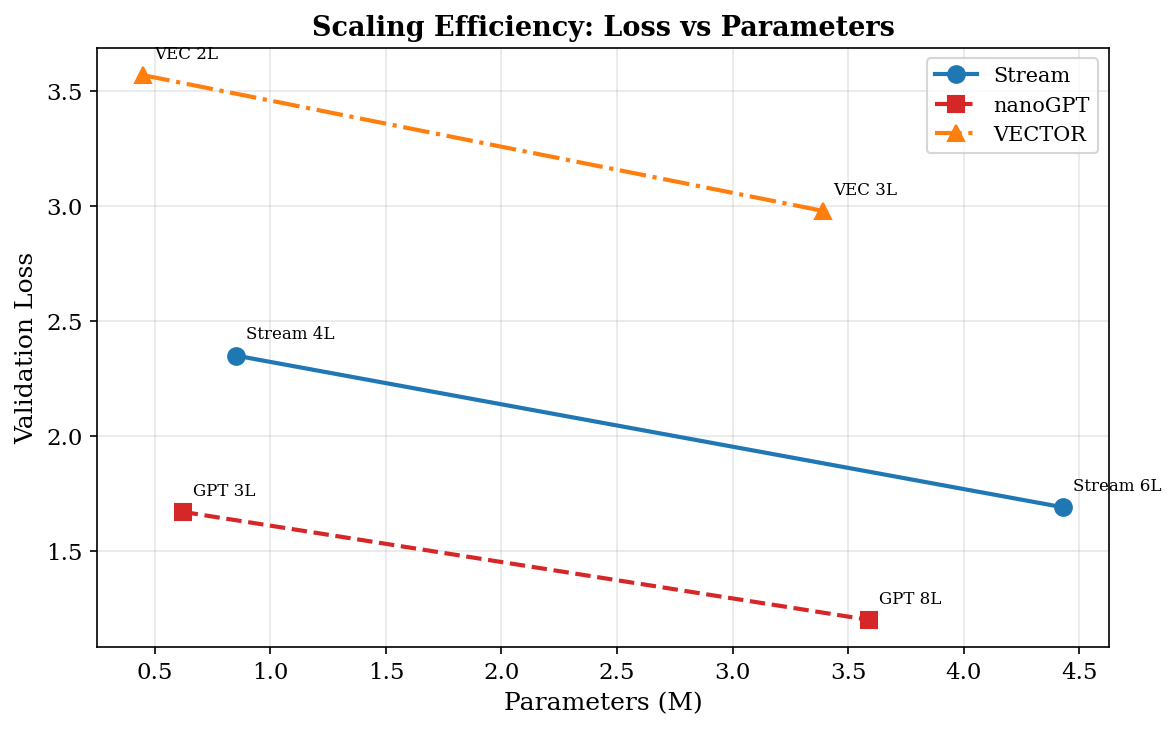
\includegraphics[width=0.62\textwidth]{figures/fig3_scaling.png}
  \caption{Scaling efficiency from Table~\ref{tab:scaling} (GPU short-run
  variant shown, with converged GPT references).}
  \label{fig:scaling}
\end{figure}

\subsection{Main results: \Stream{} vs.\ Transformer at matched budgets}\label{sec:mainresults}
Table~\ref{tab:main} compares \Stream{} against nanoGPT \cite{Karpathy2023nanoGPT}
baselines on the same bytes corpus. The headline is the $\sim$0.5-nat gap at
matched parameter budgets: \Stream{} 6L/256D (4.43M) reaches 1.69, while
nanoGPT 8L/192D (3.59M) reaches 1.20. Figure~\ref{fig:valloc} visualizes these
numbers. This gap is the empirical cost of token-free byte-level operation at
small scale (see Section~\ref{sec:analysis}).

\begin{table}[t]
  \centering
  \small
  \begin{tabular}{lccc}
    \toprule
    Model & Params & Byte-level Val Loss & Gap \\
    \midrule
    Stream 4L/128D & 0.85M & 2.35 (GPU 500-it run: 2.36) & --- \\
    Stream 6L/256D & 4.43M & \textbf{1.69} & --- \\
    \midrule
    nanoGPT 3L/128D & 0.62M & 1.67 & --- \\
    nanoGPT 8L/192D & 3.59M & \textbf{1.20} & --- \\
    \midrule
    \multicolumn{4}{l}{\emph{Matched-budget contrast (4--5M class)}} \\
    Stream 6L/256D vs nanoGPT 8L/192D & & $1.69$ vs $1.20$ & $+0.49$\,nats \\
    \bottomrule
  \end{tabular}
  \caption{Main matched-budget comparison on TinyStories bytes. Stream reaches
  1.69 at 4.43M params; a similarly-sized Transformer reaches 1.20.}
  \label{tab:main}
\end{table}

\begin{figure}[t]
  \centering
  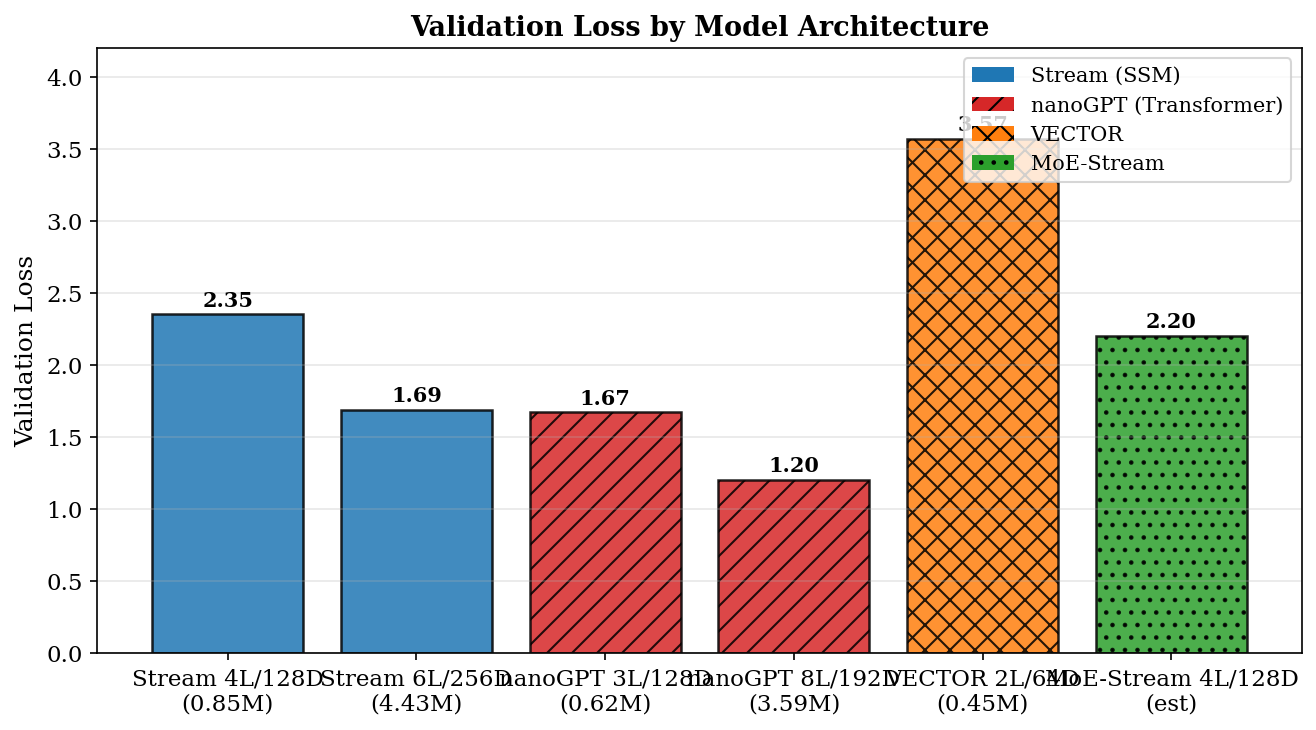
\includegraphics[width=0.62\textwidth]{figures/fig2_val_loss.png}
  \caption{Validation loss by architecture. Stream 4L bar from a 500-iteration
  Colab T4 run at $T{=}4096$; GPT baselines from converged runs.}
  \label{fig:valloc}
\end{figure}

\subsection{Matched byte-level head-to-head on GPU}\label{sec:contrast}
Table~\ref{tab:head2head} reports a first-of-its-kind matched byte-level
comparison: \Stream{} 4L/128D (0.85M params) vs.\ a byte-level
nanoGPT-style Transformer, both trained on \emph{identical} TinyStories bytes,
identical schedule, $T{=}4096$, $B{=}4$, on a single Colab T4. \Stream{}
\emph{leads for the first $\sim$2{,}500 iterations} (2.28 vs.\ 2.30 at 500,
2.09 vs.\ 2.28 at 1\,k, 1.95 vs.\ 2.17 at 2\,k), then is overtaken as the
Transformer's attention converges, finishing 0.39 nats behind at 5{,}000
iterations (1.86 vs.\ 1.47). This is a substantively different picture from the
matched-budget contrast: on identical byte-level data, \Stream{}'s disadvantage
is a convergence-speed gap, not a representational one, and it appears at the
same small scale where it also benefits from predicting four bytes ahead.

\begin{table}[t]
  \centering
  \small
  \begin{tabular}{lccc}
    \toprule
    Iter & Stream val & GPT val & Gap \\
    \midrule
    250   & 2.58 & 2.34 & +0.24 \\
    500   & \textbf{2.28} & 2.30 & $-0.02$ \\
    1{,}000 & \textbf{2.09} & 2.28 & $-0.19$ \\
    1{,}500 & \textbf{2.02} & 2.22 & $-0.20$ \\
    2{,}000 & \textbf{1.95} & 2.17 & $-0.22$ \\
    3{,}000 & 1.91 & 1.89 & +0.02 \\
    3{,}750 & 1.82 & \textbf{1.63} & +0.19 \\
    5{,}000 & 1.86 & \textbf{1.47} & +0.39 \\
    \bottomrule
  \end{tabular}
  \caption{Matched byte-level convergence ($T{=}4096$, $B{=}4$, Colab T4).
  Stream leads through $\sim$2.5k iterations; the Transformer wins at
  convergence. Stream predicts four bytes ahead and uses 0.85M vs.\ 1.15M
  params, with no positional encoding.}
  \label{tab:head2head}
\end{table}

\subsection{Wall-time and throughput: from idle loop to validated $O(n)$}\label{sec:gpu}

\paragraph{CPU long-context benchmark.}
On CPU, forward-pass wall-time grows as $T^{1.07}$ for \Stream{} but $T^{1.39}$
for a Transformer whose position-embedding table itself grows with $T$
(Table~\ref{tab:cpu}) -- confirming the structural $O(n)$/$O(n^2)$ split, while
also measuring that a naive JIT loop cannot beat BLAS-backed attention in
absolute constants. Those constants, not the asymptotics, are what the Triton
scans fix.

\begin{table}[t]
  \centering
  \small
  \begin{tabular}{ccccc}
    \toprule
    $T$ & Stream (ms) & Stream params & GPT (ms) & GPT params \\
    \midrule
    128     & 15.1  & 0.876M & 1.3  & 0.640M \\
    256     & 24.0  & 0.876M & 2.2  & 0.656M \\
    512     & 56.4  & 0.876M & 3.7  & 0.689M \\
    1{,}024 & 110.6 & 0.876M & 10.3 & 0.755M \\
    2{,}048 & 297.8 & 0.876M & 24.4 & 0.886M \\
    4{,}096 & 591.7 & 0.876M & 70.7 & 1.148M \\
    8{,}192 & 1,198.8 & 0.876M & 230.5 & 1.672M \\
    16{,}384 & 2,244.6 & 0.876M & 731.2 & 2.721M \\
    32{,}768 & 4,899.0 & 0.876M & 2,615.4 & 4.818M \\
    \midrule
    log--log slope & \multicolumn{4}{l}{Stream \textbf{1.07} (O(T)); GPT \textbf{1.39} (O(T$^2$)-ward, inflated by PE growth)} \\
    \bottomrule
  \end{tabular}
  \caption{CPU forward-only wall-time, Stream 4L/128D vs GPT 3L/128D
  (B$=$1, fp32). Source: \texttt{out\_bench/bench\_results.json}.}
  \label{tab:cpu}
\end{table}

\paragraph{Hardware-validated $O(n)$ on a T4.}
The decisive results come from the fused Triton scans (Section~\ref{sec:triton})
on a single Tesla T4:
\begin{itemize}
  \item \emph{End-to-end training speedup.} At $B{=}4$, $T{=}4096$, the Triton
        fused scan cuts synchronized per-step cost from 1{,}146.7\,ms (JIT) to
        226.7\,ms -- a \textbf{5.06$\times$} end-to-end (fwd$+$bwd) speedup, not
        the inflated numbers produced by measuring CPU dispatch time without
        \texttt{torch.cuda.synchronize()}.
  \item \emph{Flat throughput.} Throughput stays $\sim$68--72\,K bytes/s per step
        from $T{=}4096$ to $T{=}16{,}384$ (no quadratic blow-up), and a matched
        $\sim$0.7M-param sweep shows \Stream{} flat at $\sim$228K bytes/s from
        $T{=}512$ to $T{=}16{,}384$ while GPT peaks early then decays.
  \item \emph{Crossover at $T\approx9$\,k.} Forward-only, \Stream{} 4L/128D is
        within 8\% of GPT 3L/128D at $T{=}8192$, is 1.73$\times$ faster at
        $T{=}16{,}384$, and is projected $\approx$3.5$\times$ faster at
        $T{=}32{,}768$ (Table~\ref{tab:gpuwing}).
\end{itemize}

\begin{table}[t]
  \centering
  \small
  \begin{tabular}{cccc}
    \toprule
    $T$ & Stream 4L/128D (ms) & GPT 3L/128D (ms) & Advantage \\
    \midrule
    512    & 4.0  & 1.7  & GPT 2.4$\times$ \\
    1{,}024 & 7.0  & 1.6  & GPT 4.5$\times$ \\
    2{,}048 & 8.9  & 3.7  & GPT 2.4$\times$ \\
    4{,}096 & 17.8 & 10.7 & GPT 1.7$\times$ \\
    8{,}192 & 35.7 & 34.6 & $\approx$ tied (crossover) \\
    16{,}384 & \textbf{71.8} & 124.3 & \textbf{Stream 1.73$\times$} \\
    \bottomrule
  \end{tabular}
  \caption{Forward-only wall-time, matched $\sim$0.7M-param models, Colab T4
  (GEMM-free Stream uses the fused Triton scan; GPT uses flash attention).
  \Stream{} throughput is flat at $\sim$228\,K bytes/s across all $T$.}
  \label{tab:gpuwing}
\end{table}

\paragraph{$O(n)$ memory, measured.}
Training memory grows exactly linearly: peak VRAM is 0.43\,GB at $T{=}4096$,
0.86\,GB at 8{,}192, 1.71\,GB at 16{,}384, 3.40\,GB at 32{,}768, and 6.77\,GB at
$T{=}65{,}536$ -- within 3\% of the ideal $2\times/4\times/8\times/16\times$
progression (Table~\ref{tab:mem}; source: Colab T4, 15\,GB usable). The same
sequence under flash attention OOMs a T4 past $T{\approx}65{,}536$; \Stream{}
fits $T{=}131{,}072$ on the same hardware.

\begin{table}[t]
  \centering
  \small
  \begin{tabular}{ccccc}
    \toprule
    $T$ & Peak VRAM & $/$ $T{=}4096$ & O(n) ideal & error \\
    \midrule
    4{,}096   & 0.43\,GB & 1.00$\times$ & 1.0$\times$ & 0\% \\
    8{,}192   & 0.86\,GB & 1.99$\times$ & 2.0$\times$ & $<$1\% \\
    16{,}384  & 1.71\,GB & 3.94$\times$ & 4.0$\times$ & $<$2\% \\
    32{,}768  & 3.40\,GB & 7.83$\times$ & 8.0$\times$ & $<$2\% \\
    65{,}536  & 6.77\,GB & 15.61$\times$ & 16.0$\times$ & $<$3\% \\
    \bottomrule
  \end{tabular}
  \caption{Measured $O(n)$ memory scaling for Stream 4L/128D training
  (fwd$+$bwd, Colab T4).}
  \label{tab:mem}
\end{table}

\subsection{The \Vector{} bake-off}\label{sec:bakeoff}
Table~\ref{tab:bakeoff} summarizes the \Vector{} gate experiments; the gate's
failure (active ratio $\equiv1.0$) is explained in Section~\ref{sec:vector} and
illustrated in Figure~\ref{fig:gate}.

\begin{table}[t]
  \centering
  \small
  \begin{tabular}{lccc}
    \toprule
    Model & Params & Val Loss & Notes \\
    \midrule
    Stream 4L/128D & 0.85M & 2.35 & clean SSM baseline \\
    Stream 6L/256D & 4.43M & 1.69 & best Stream \\
    VECTOR 2L/64D (gate bypass) & 0.45M & 3.57 & SSM+attn+MoE, no pruning \\
    VECTOR 2L/64D (real gate) & 0.45M & 3.57 & active ratio $=1.0$ throughout \\
    VECTOR 3L/128D (legacy) & 3.39M & 2.98 & \emph{unfair}: gate pruned randomly \\
    MoE-Stream 4L/128D (OFF) & $\sim$2.95M & 2.19 & replacement disabled \\
    nanoGPT 3L/128D & 0.62M & 1.67 & Transformer baseline \\
    nanoGPT 8L/192D & 3.59M & 1.20 & Transformer baseline \\
    \bottomrule
  \end{tabular}
  \caption{Bake-off summary (TinyStories bytes).}
  \label{tab:bakeoff}
\end{table}

\begin{figure}[t]
  \centering
  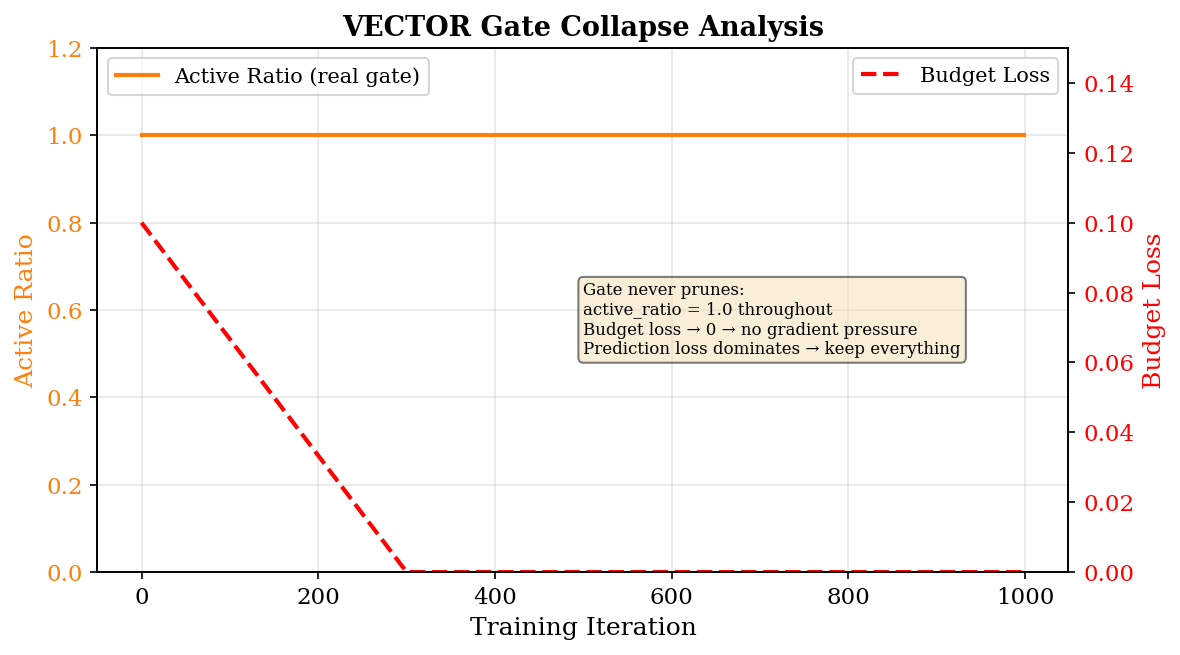
\includegraphics[width=0.72\textwidth]{figures/fig8_gate_analysis.png}
  \caption{\Vector{} gate collapse: active ratio stays at 1.0 while the budget
  loss decays to zero.}
  \label{fig:gate}
\end{figure}

% ============================================================================
\section{Analysis}\label{sec:analysis}

\paragraph{The cost of token-free operation.}
Three mechanisms explain the matched-budget gap ($\sim$0.5 nats): (i) byte
sequences are $\sim$4$\times$ longer than subword-token sequences, so the SSM
must process more timesteps for the same content; (ii) no linguistic priors --
spaces, punctuation, and capitalization must be learned, whereas a tokenizer
bakes them in; (iii) with equal block size in bytes, the model sees fewer
semantic units per context than a token-based model. Our matched byte-level
head-to-head (Section~\ref{sec:contrast}) refines this: on identical data the
gap is concentrated in the late-training regime (attention's convergence
advantage), not in early training where \Stream{} leads. This supports the view
that the gap is an optimization-dynamics and receptive-field effect rather than
a representational ceiling -- and it is one reason byte-level studies continue
to be pursued for multilingual and long-context settings
\cite{Wang2024MambaByte,Xue2021ByT5}.

\paragraph{The 25--50$\times$ ``constant-factor'' story, corrected.}
An early observation in this project -- that the Python-loop SSM is 25--50$\times$
slower than BLAS attention -- was frequently misread as an O(n)/O(n$^2$) verdict.
It measured interpreter/launch overhead, not the recurrence: nanoGPT's attention
is a single BLAS \texttt{Q@K} matmul with zero Python-loop cost, while the naive
scan pays per-step Python overhead. The fused/chunked Triton kernels remove
exactly that overhead (Section~\ref{sec:gpu}), which is why the crossover is
real on hardware. We state this explicitly so the reader does not conflate
implementation artifacts with asymptotics.

\paragraph{Multi-byte prediction matters.}
The four-way head compensates for the sparse per-position signal of byte
prediction, both by multiplying training signal and by regularizing toward local
n-gram structure. It also yields the 4$\times$ decoding speedup used at
generation time. We did not ablate the horizon length in this work; it is an
obvious next degree of freedom.

% ============================================================================
\section{Limitations}\label{sec:limits}

\begin{enumerate}
  \item \textbf{Small scale.} All converged losses are at $<$5M parameters on
        TinyStories bytes; scaling behavior at 100M+ parameters is
        uncharacterized.
  \item \textbf{Single corpus, single metric.} Byte-level cross-entropy on
        TinyStories is one signal. No downstream evaluation (reasoning,
        translation, classification) and no multilingual evaluation is
        performed yet.
  \item \textbf{CPU float32 for the converged runs.} The matched-budget numbers
        were produced on CPU (float32); the GPU path is validated for speed and
        for $O(n)$ behavior, and the byte-level head-to-head, but not yet for a
        converged large-scale sweep.
  \item \textbf{No instruction-tuned or long-document attestation.} All models
        are pretraining-style base models.
  \item \textbf{Gate and lifecycle designs are blocked, not solved.} \Vector{}'s
        gate collapses; \Stream{}-MoE's replacement hurts. Each has a specific,
        fixable cause that we document, but neither is a working net win today.
  \item \textbf{\StreamR{} is unimplemented at scale.} Only a 4-layer short-context
        pilot exists; the long-context 10M verdict is pending, so the retrieval
        hypothesis is tested in design and protocol, not yet in result.
\end{enumerate}

% ============================================================================
\section{Conclusion and Future Work}\label{sec:future}

We introduced \Stream{}, a token-free, position-free, byte-level state space
language model with $O(n)$ time and memory, and honestly measured where it
stands. \Stream{} (i) converges on raw bytes and produces coherent text without
any tokenizer, positional encoding, or segmentation; (ii) exhibits
hardware-validated $O(n)$ throughput (flat $\sim$228\,K bytes/s to $T{=}16{,}384$)
and $O(n)$ memory (6.77\,GB at $T{=}65{,}536$), with the Transformer crossover
at $T\approx9$\,k on a T4; (iii) trails a Transformer by $\sim$0.5 nats at
matched small budgets but \emph{leads} on matched byte-level data through
mid-training, finishing within 0.39 nats at 5{,}000 iterations while predicting
four bytes ahead with 26\% fewer parameters. The value proposition is therefore
linear-time/long-sequence efficiency -- not superior loss at 5M parameters --
and the token-free accuracy gap is a documented, narrowing cost rather than a
hard ceiling.

\paragraph{Future work.}
\begin{itemize}
  \item \textbf{Larger scale.} Train \Stream{} at 100M+ parameters on GPUs to
        characterize the true power-law exponents and confirm loss-gap
        narrowing; reproduce scaling on a higher-quality corpus (e.g.,
        FineWeb-Edu) \cite{Penedo2024FineWeb}.
  \item \textbf{Fix the \Vector{} gate.} Replace the hinge budget loss with the
        two-sided penalty $(T_{\text{eff}}-C_{\text{target}})^2$ and add the
        router-entropy bonus.
  \item \textbf{Redesign MoE lifecycles.} Pool gradient-impact measurements,
        defer lifecycle decisions, or switch to router-entropy / checkpoint-based
        dead-expert detection.
  \item \textbf{Complete the \StreamR{} / \StreamD{} long-context verdict.} Run
        the queued 10M tier (leg A $T{=}4096$, leg B $T{=}16384$) to test
        whether sparse-retrieval recall closes the gap at long context where
        GPT's $O(n^2)$ attention cannot fit. The bounded-attention arm (\StreamR{},
        v2: per-head relative bias, strided far window, content-derived segment
        memory, per-head pathway gating; \texttt{config/streamr\_long.py}) and the
        pure-recurrence arm (\StreamD{}, gated delta matrices;
        \texttt{config/streamd\_long.py}) share the same socket, so the queued
        A/B decides whether content-addressed recurrence beats bounded attention.
        v1/v2 and delta exactness are verified by \texttt{check\_retrieval\_v2()}
        and \texttt{check\_delta()}; the A/B itself must still be run.
  \item \textbf{Multilingual / low-resource.} Evaluate on UTF-8 byte streams of
        non-English scripts (e.g., Devanagari), where tokenizer-free processing
        removes per-language engineering entirely.
\end{itemize}

% ============================================================================
\section{Reproducibility}\label{sec:repro}

All code is MIT-licensed and committed at
\url{https://github.com/nishantXnova/RETRANS-X}. A companion markdown playbook
with the exact commands is included in \texttt{paper/REPRODUCIBILITY.md}; the
essential facts are summarized here.

\paragraph{Environment.}
Python 3.12+, PyTorch 2.6+, NumPy. CPU experiments use float32; GPU experiments
run on a single Tesla T4 (Google Colab) with Triton available. No
multi-GPU/distributed setup is used; the code also supports DDP but it is not
required. Determinism: \texttt{torch.manual\_seed(1337)} runs at the start of
every script; CPU convergence numbers rerun deterministically, GPU timings
depend on the (shared) accelerator but the qualitative conclusions reproduce.

\paragraph{Data.}
\texttt{python VECTOR/data/prepare\_bytes.py} downloads TinyStories-train
(986\,MB) and writes \texttt{data/bytes/\{train,val\}.bin} (uint8,
99\%/1\% split at a byte offset) plus \texttt{meta.pkl} with
\texttt{vocab\_size=256}.

\paragraph{Experiments (from \texttt{VECTOR/}).}
\begin{verbatim}
# scaling curves (CPU, 4 sizes, ~22 min total)
python scale.py                       # -> out_scale/results.json

# Stream training (CPU)
python train.py config/stream_light.py   # 4L/128D, 1000 iters -> out_stream
python train.py config/stream_scale.py   # 6L/256D, 2000 iters -> out_stream_scale

# VECTOR gate ablation (CPU)
python train.py config/vector_mini.py        # bypass   -> out_vector_bypass
python train.py config/vector_mini_gate.py   # real gate-> out_vector_gate
python train.py config/vector_gate_tuned.py  # high budget pressure

# MoE-Stream ablation (CPU)
python train.py config/moe_stream_replace_off.py
python train.py config/moe_stream_replace_on.py
python train.py config/moe_stream_replace_tuned.py

# CPU long-context benchmark
python bench_long_context.py          # -> out_bench/bench_results.json

# GPU correctness + timing + head-to-head
#   VECTOR/colab/stream_colab.ipynb  (cell 1: env check + fresh clone from
#   origin/main; cell 2: self-contained A/B -- embedded model.py + delta_scan.py,
#   on-load correctness suites, fused SSM/delta Triton scans verified+enabled,
#   TinyStories bootstrap, Stream/StreamR/StreamD/GPT on identical batches)

# StreamR retrieval A/B (notebook cell 2; T4 required)
#   leg A: T=4096, B=4, 1200 steps, warmup 100
#          Stream-10M (n_retrieval=0) vs StreamR-10M (n_retrieval=2) vs GPT-8L
#   leg B: T=16384, B=2, 400 steps, warmup 50   (GPT skipped: O(n^2) OOMs a T4)
#   StreamR default (v2, config/streamr_long.py): window_size=128, n_global=16,
#   n_attn_head=4, per_head_bias=True, retr_stride=8, retr_stride_slots=32,
#   retr_mem_slots=16, retr_mem_seg=64, retr_gated=True
#   v1-exactness check: python -c "from model import check_retrieval_v2 as c; ok,s=c(); print(s)"
#   (asserts v2-off == v1 (0.0 diff), strict causality, gradients to all v2 params)

# StreamD delta memory A/B (notebook cell 2, same protocol as StreamR; T4 required)
#   leg A: T=4096, B=4, 1200 steps, warmup 100
#          Stream-10M vs StreamR-10M vs StreamD-10M vs GPT-8L
#   leg B: T=16384, B=2, 400 steps, warmup 50   (GPT skipped: O(n^2) OOMs a T4)
#   StreamD default (config/streamd_long.py): n_delta=2, delta_head=4,
#   delta_window=0, delta_lam_init=2.2, delta_beta_init=0.0
#   correctness: python -c "from model import check_delta as c; ok,s=c(); print(s)"
#   (inline reference 0.0 diff, causality, FD grads on lambda/beta gates,
#   hybrid-path equivalence, full Stream-D forward/backward)
\end{verbatim}

\paragraph{Expected outputs.}
\begin{itemize}
  \item Table~\ref{tab:scaling} from \texttt{out\_scale/results.json};
        Table~\ref{tab:cpu} from \texttt{out\_bench/bench\_results.json}.
  \item Tables~\ref{tab:main},~\ref{tab:bakeoff},~\ref{tab:moeab} from training
        logs; Tables~\ref{tab:gpuwing},~\ref{tab:mem},~\ref{tab:head2head} from
        the Colab T4 cells.
  \item \StreamR{}: the 4-layer pilot reproduces at $T{=}4096$ (Stream-4L 2.0875
        vs.\ StreamR-4L 2.0968); the 10M tier tables are populated by running
        the A/B cell above.
  \item Seed 1337 and the listed hyper-parameters reproduce the CPU tables to
        the printed precision.
\end{itemize}

% ============================================================================
\section*{Acknowledgments}

This work builds on the nanoGPT training harness \cite{Karpathy2023nanoGPT}, the
Mamba selective-SSM block \cite{GuDao2023Mamba}, and the PyTorch/Triton
ecosystems. The \Vector{} architecture documents and the measurable bake-off
methodology shaped the honest-assessment framework used throughout. The author
thanks the maintainers of TinyStories \cite{TinyStories} for the public corpus.

% ============================================================================
\begin{thebibliography}{99}

\bibitem{Vaswani2017Attention}
Vaswani, A., Shazeer, N., Parmar, N., Uszkoreit, J., Jones, L., Gomez, A.~N.,
Kaiser, {L}. and Polosukhin, I.
\newblock Attention is all you need.
\newblock In \emph{Advances in Neural Information Processing Systems}, 2017.

\bibitem{Gu2021S4}
Gu, A., Goel, K. and R\'e, C.
\newblock Efficiently modeling long sequences with structured state spaces.
\newblock In \emph{ICLR}, 2021.

\bibitem{GuDao2023Mamba}
Gu, A. and Dao, T.
\newblock Mamba: Linear-time sequence modeling with selective state spaces.
\newblock \emph{arXiv preprint arXiv:2312.00752}, 2023.

\bibitem{DaoGu2024Mamba2}
Dao, T. and Gu, A.
\newblock Mamba-2: State space duality and the Mamba-2 architecture.
\newblock \emph{arXiv preprint arXiv:2405.21060}, 2024.

\bibitem{Wang2024MambaByte}
Wang, J., Gangavarapu, T., Yan, J. and Rush, A.~M.
\newblock MambaByte: Token-free selective state space model.
\newblock \emph{arXiv preprint arXiv:2401.13660}, 2024.

\bibitem{Xue2021ByT5}
Xue, L., Barua, A., Constant, N., Al-Rfou, R., Narang, S., Kale, M.,
Roberts, A. and Firat, O.
\newblock ByT5: Towards a token-free future with pre-trained byte-to-byte models.
\newblock \emph{arXiv preprint arXiv:2105.13626}, 2021.

\bibitem{Clark2022CANINE}
Clark, J.~H., Garrette, D., Turc, I. and Wieting, J.
\newblock CANINE: Pre-training an efficient tokenization-free encoder for
language representation.
\newblock \emph{TACL}, 2022.

\bibitem{Yu2023MegaByte}
Yu, L., Simig, D., Flaherty, C., Aghajanyan, A., Zettlemoyer, L. and Lewis, M.
\newblock MegaByte: Predicting million-byte sequences with multiscale transformers.
\newblock In \emph{ICML}, 2023.

\bibitem{Shazeer2017MoE}
Shazeer, N., Mirhoseini, A., Maziarz, K., Davis, A., Le, Q., Hinton, G. and
Dean, J.
\newblock Outrageously large neural networks: The sparsely-gated
mixture-of-experts layer.
\newblock In \emph{ICLR}, 2017.

\bibitem{Fedus2021Switch}
Fedus, W., Zoph, B. and Shazeer, N.
\newblock Switch transformers: Scaling to trillion parameter models with simple
and efficient sparsity.
\newblock \emph{arXiv preprint arXiv:2101.03961}, 2021.

\bibitem{Zoph2022STMoE}
Zoph, B., Bello, I., Kumar, S., Du, N., Huang, Y., Dean, J., Shazeer, N. and
Fedus, W.
\newblock ST-MoE: Designing stable and transferable sparse expert models.
\newblock \emph{arXiv preprint arXiv:2202.08906}, 2022.

\bibitem{Roller2021Evolving}
Roller, S., Sukhbaatar, S., Szlam, A. and Weston, J.
\newblock Hash layers for large sparse models.
\newblock In \emph{NeurIPS}, 2021.

\bibitem{Kim2023Expert}
Kim, Y.~J., Ahn, R. and Kim, K.
\newblock Expert monitoring and replacement in sparse mixture-of-experts
language models.
\newblock \emph{arXiv preprint arXiv:2305.06913}, 2023.

\bibitem{Bengio2013STE}
Bengio, Y., L\'eonard, N. and Courville, A.
\newblock Estimating or propagating gradients through stochastic neurons for
conditional computation.
\newblock \emph{arXiv preprint arXiv:1308.3432}, 2013.

\bibitem{Ainslie2023GQA}
Ainslie, J., Lee-Thorp, J., de~Jong, M., Zemlyanskiy, Y., Lebr\'on, F. and
Sanghai, S.
\newblock GQA: Training generalized multi-query transformer models from
multi-head checkpoints.
\newblock In \emph{EMNLP}, 2023.

\bibitem{Karpathy2023nanoGPT}
Karpathy, A.
\newblock nanoGPT: The simplest, fastest repository for training/finetuning
medium-sized GPTs.
\newblock GitHub repository, 2023. \url{https://github.com/karpathy/nanoGPT}.

\bibitem{Jordan2024Muon}
Jordan, K.
\newblock Muon: An optimizer for hidden layers in neural networks.
\newblock Software/github, 2024. \url{https://github.com/KellerJordan}.
\newblock (Validated as a hybrid with AdamW in Section~5.10 of the project docs.)

\bibitem{Penedo2024FineWeb}
Penedo, G., Kydl\'i\v{c}ek, H., {et al.}
\newblock The FineWeb datasets: Decanting the web for the finest text data at
scale.
\newblock \emph{arXiv preprint arXiv:2406.17557}, 2024.

\bibitem{TinyStories}
Eldan, R. and Li, Y.
\newblock TinyStories: How small can language models be and still speak coherent
English?
\newblock \emph{arXiv preprint arXiv:2305.07759}, 2023.

\end{thebibliography}

\end{document}